% One-page summary. Figures: python report/make_figures.py   Build: tectonic report/summary.tex
\documentclass[a4paper,10pt,twocolumn]{article}
\usepackage[margin=1.25cm,top=1.1cm,bottom=1.1cm,columnsep=0.6cm]{geometry}
\usepackage[T1]{fontenc}
\usepackage{lmodern,microtype,graphicx,booktabs,enumitem,xcolor}
\usepackage[compact]{titlesec}
\titleformat{\section}{\normalsize\bfseries\color[HTML]{2a78d6}}{}{0pt}{}
\titlespacing*{\section}{0pt}{5pt}{2pt}
\setlist{nosep,leftmargin=*,itemsep=1pt}
\setlength{\parindent}{0pt}
\setlength{\parskip}{3pt}
\graphicspath{{figures/}}
\pagestyle{empty}

\begin{document}
\twocolumn[{%
  {\Large\bfseries Bringing the Heat: day-ahead demand forecasts for heat-pump homes}\\[2pt]
  {\small Pengxuan Huang \textperiodcentered{} Xinran Ge \textperiodcentered{} Giorgio Checola \textperiodcentered{} Ahsen Uluta\c{s} \textperiodcentered{} Hiba Naeem}\\[4pt]
  \small\textbf{Task:} forecast how much electricity 375 heat-pump households will draw from the grid on the next day, so E.ON can buy the right amount on the day-ahead market.
  \textbf{Result:} one gradient-boosting model for all households predicts each household's daily demand with a \textbf{mean absolute error of 5.8\,kWh} (average demand 26.9\,kWh per day) and \textbf{$R^2 = 0.82$}. For all households combined, the daily error is 7.8\,\% ($R^2 = 0.94$).\\[3pt]
  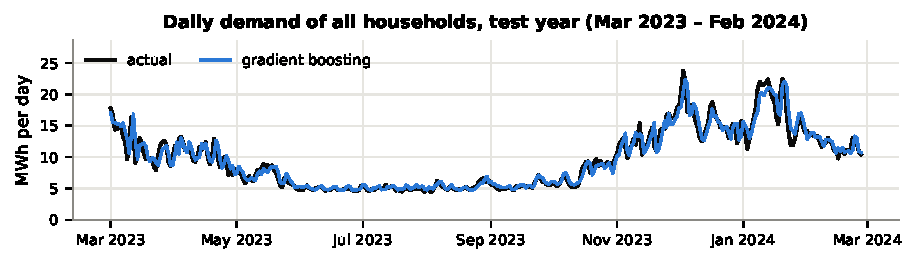
\includegraphics[width=\textwidth]{daily_demand.pdf}\\[2pt]
}]

\small
\section{Data and setup}
\begin{itemize}
  \item \textbf{Data:} 15-min grid consumption of 375 households with $>1$ year of data and survey metadata (118 with PV, 99 without, 158 unknown), 8 hourly weather stations.
  \item \textbf{Cleaning:} columns read by name (their order differs between files); missing and impossible readings ($>40$\,kW) dropped, never imputed; weather timestamps mark the \emph{end} of the hour and are shifted; sunshine for the 3 stations without a sensor is filled from the other stations and flagged.
  \item \textbf{Day-ahead rule:} the forecast for day D only uses data up to the end of day D$-$1 (yesterday's load and weather, the load one week earlier). Nothing from day D.
  \item \textbf{Split by time:} train before 1 March 2023, \textbf{test on the following 12 months} (to evaluate effectiveness for entire year). Hyperparameters tuned on Jan--Feb 2023, never on the test year.
\end{itemize}

\section{Model (Level 0)}
One \textbf{global gradient-boosting model} GBM for all households with 26 features: load of the same 15 min yesterday and one week earlier, yesterday's weather, time of day, weekday, month, PV flag, heat-pump optimisation visit and building survey answers. Most important (permutation importance): yesterday's and last week's load, yesterday's mean temperature, living area, time of day. A hyperparameter search on Jan--Feb 2023 kept the default settings.

\section{Results: daily demand per household, test year}
\begin{tabular}{@{}lcc@{}}
\toprule
Model & MAE (kWh per day) & $R^2$ \\
\midrule
\textbf{Gradient boosting} & \textbf{5.79} & \textbf{0.819} \\
Baseline: same day last week & 7.87 & 0.631 \\
\bottomrule
\end{tabular}

\vspace{3pt}
The baseline repeats each household's demand from the same day one week earlier. Gradient boosting \textbf{cuts the daily error by 26\,\%} (7.87 $\rightarrow$ 5.79\,kWh) and raises $R^2$ from 0.63 to 0.82, because it learns how demand reacts to temperature, time of day and household characteristics. Without a weather forecast for day D, it still reacts to weather changes about a day late (see the cold snaps in the chart above). For all households combined, the errors largely cancel: the daily error is 750\,kWh on an average of 9.6\,MWh (7.8\,\%).

\section{PV vs no PV (Level 1)}
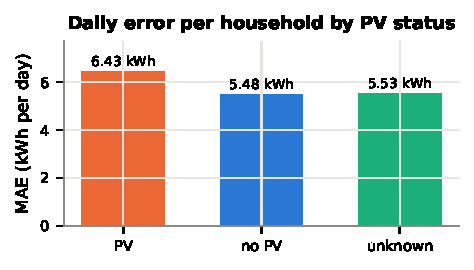
\includegraphics[width=\columnwidth]{pv_groups.pdf}
PV households have a $\approx$\,17\,\% higher daily MAE (6.43 vs 5.48\,kWh): their grid draw depends on the next day's sunshine, which the model only knows from yesterday. Unknown-status households behave like no-PV ones.

\section{Uncertainty and buying decision (Levels 2--3)}
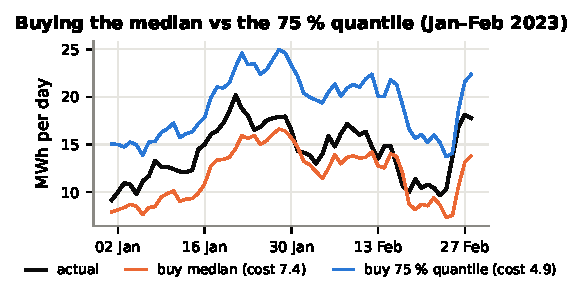
\includegraphics[width=\columnwidth]{quantile_buying.pdf}
Quantile gradient boosting: 80\,\% intervals contain 78\,\% of the readings (Jan--Feb 2023 validation). If buying too little costs \textbf{3$\times$} more than buying too much, the optimal amount is the 75\,\% quantile ($3/(3+1)$). Buying it instead of the median \textbf{cuts the daily cost by 34\,\%}; summed household medians fall short on 56 of 59 days.

\section{Limitations and next steps}
\begin{itemize}
  \item \textbf{No weather forecasts in the data:} with day D's measured weather as a perfect forecast, the daily error dropped from 11.3\,\% to 4.2\,\% in an earlier experiment. A real weather forecast is the biggest lever.
  \item Next: quantiles of the \emph{total} demand (summed household quantiles over-buy), PV-specific models, real market prices.
\end{itemize}
\end{document}
